\section{Research Idea 5: Explicit Geometry and Human Pose for Social-Norm Reasoning}
\subsection{Initial Implementation}
\label{sec:idea5-impl}

\paragraph{Task and inputs.}
EgoNormia asks for the normatively appropriate next action in an egocentric clip and its justification; each head has five options plus ``None of these'', which is never gold on our test set. We report \emph{joint accuracy} (both heads correct) on the 200 verified items $T$; training and cross-validation use 600 further items from disjoint source videos. Each item is given as a strip of five pre-action RGB frames, the same frames rendered as depth (Depth-Anything-V2-Small), instance segmentation (YOLOv8n-seg) and body/hand skeleton (MediaPipe) maps, and one spatial description per image written by Gemini~4 without access to the question. The same extractors yield four spatial labels per item (people count, nearest-person distance, facing, hands visible).

\paragraph{Controls.}
Every spatial arm has a matched control with the same amount of non-spatial content: maps and descriptions from another item (\emph{mismatched}), the RGB strip repeated, EgoNormia's own non-spatial scene description, or, for training, an identical LoRA on non-spatial data. A \emph{spatial-specific} effect is a spatial arm minus its matched control; a gain over RGB alone is not evidence of spatial transfer.

\paragraph{Universal embedding.}
Qwen3-VL-Embedding-8B (frozen) encodes the context as one L2-normalised vector $\mathbf c$ and each option as $\mathbf o$. Conditions are C2 (RGB + its description), C5 (C2 followed by each map and its description, our combined embedding), X1 (C5 with another item's maps and descriptions) and X3 (C2 with the strip repeated). A low-rank bilinear scorer with an option prior and an abstention bias,
\begin{equation}
s(\mathbf c,\mathbf o)=\alpha\,\mathbf c^{\top}\mathbf o+(A\mathbf c)^{\top}(B\mathbf o)+\mathbf v^{\top}\mathbf o+\beta\,\mathbf{1}[o=\text{None}],
\end{equation}
is trained with softmax cross-entropy over each head $h\in\{a,j\}$,
\begin{equation}
\begin{split}
\mathcal L_{\mathrm{sc}}={}&-\tfrac1N\textstyle\sum_{i}\sum_{h}\log p\big(y^{h}_i\mid\mathbf c_i,O^{h}_i\big)\\
&+\lambda\big(\|A\|_F^2+\|B\|_F^2+\|\mathbf v\|^2\big),
\end{split}
\end{equation}
evaluated by 5-fold CV grouped by source video (800 items) and on $T$. A logistic probe on $\mathbf c$ measures whether the spatial labels are linearly readable (balanced accuracy); since the labels come from the map extractors, it is a manipulation check rather than an independent spatial measure.

\paragraph{Direct answering.}
Gemini~4, GPT-5.6 and Qwen3-VL-32B answer from RGB alone, plus maps, plus mismatched maps, RGB repeated, plus descriptions, text-only descriptions (reworded vs.\ \emph{spatially reversed}, with every left/right, near/far and toward/away flipped), spatial vs.\ generic chain-of-thought, and forced choice with ``None'' removed.

\paragraph{Spatial fine-tuning.}
Qwen3-VL-8B is LoRA-tuned ($r{=}16$) with $\mathcal L_{\mathrm{SFT}}=-\sum_{t\in\text{ans}}\log\pi_\theta(y_t\mid x,y_{<t})$ on 5,000 SAT spatial QA items, against an identical LoRA on 5,000 VQAv2 items with spatial words removed (two seeds each). We also compare four published spatial fine-tunes with their bases: SpatialLadder-3B and MindCube-RL-3B (Qwen2.5-VL-3B), SpaceR-7B and Spatial-SSRL-7B (Qwen2.5-VL-7B).

\paragraph{Statistics.}
Contrasts are paired over items: exact McNemar tests on joint correctness and 95\% percentile-bootstrap CIs (resampling items, or source videos for CV). Ten spatial-specific contrasts are pooled with DerSimonian--Laird random effects.

\subsection{Results and Discussion}
\label{sec:idea5-results}

No spatial intervention improved social-norm accuracy beyond its matched control. The pooled spatial-specific effect is $+0.2\ [-1.7,+2.1]$ percentage points (pp); spatial \emph{training} is harmful (SAT LoRA $-6.5\ [-12.0,-1.0]$ against a matched non-spatial LoRA), and the only positive family is text-only reversal ($+3.5\ [+0.9,+6.0]$), where spatial content is the sole evidence (Table~\ref{tab:idea5-contrasts}, Figure~\ref{fig:forest}).

\begin{table}[t]
\caption{Key contrasts on EgoNormia joint accuracy ($\Delta$ in pp, 95\% bootstrap CI, exact McNemar $p$).}
\label{tab:idea5-contrasts}
\centering
\small
\setlength{\tabcolsep}{2pt}
\begin{tabular}{@{}lr@{\;}lr@{}}
\toprule
Contrast & \multicolumn{2}{l}{$\Delta$ [95\% CI]} & $p$ \\
\midrule
\multicolumn{4}{@{}l}{\textit{Embedding scorer (CV, $n{=}799$)}} \\
C5 $-$ C2 & $+2.6$ & $[+0.4,+4.9]$ & \\
C5 $-$ X1 (mismatched) & $+1.3$ & $[-0.9,+3.4]$ & \\
\multicolumn{4}{@{}l}{\textit{Direct answering (3 models pooled)}} \\
Maps $-$ mismatched maps & $-0.7$ & $[-3.2,+1.8]$ & \\
Maps $-$ RGB repeated & $+2.8$ & $[+0.3,+5.2]$ & \\
Text: reworded $-$ reversed & $+3.5$ & $[+0.9,+6.0]$ & \\
\multicolumn{4}{@{}l}{\textit{Spatial training}} \\
SAT LoRA $-$ control LoRA & $-6.5$ & $[-12.0,-1.0]$ & \\
SpatialLadder-3B $-$ base & $-12.0$ & $[-19.5,-4.5]$ & .003 \\
SAT LoRA+maps $-$ base & $-9.8$ & $[-16.5,-3.2]$ & ${<}.001$ \\
\midrule
All spatial-specific ($k{=}10$) & $+0.2$ & $[-1.7,+2.1]$ & \\
\bottomrule
\end{tabular}
\end{table}

\begin{figure}[t]
\centering
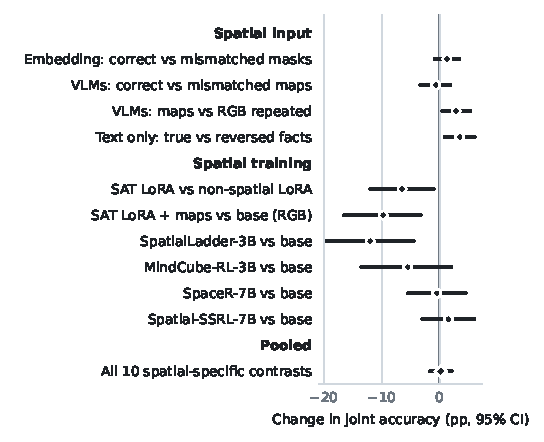
\includegraphics[width=\columnwidth]{forest_compact}
\caption{Key contrasts (change in joint accuracy, pp, 95\% CI). Spatial input is null against matched controls and spatial training is neutral to harmful; pooled spatial-specific effect $+0.2\ [-1.7,+2.1]$.}
\label{fig:forest}
\end{figure}

\paragraph{Spatial input.}
The combined embedding makes geometry more readable (probe C5 $-$ C2 $+3.4\ [+2.2,+4.7]$; facing $+7.6$, hands $+4.3$) and gives a small social gain over C2 ($+2.6$), but not over mismatched masks ($+1.3\ [-0.9,+3.4]$): extra input helps, correct geometry does not. Direct answering shows the same pattern. Maps raise accuracy (GPT-5.6 68.5$\to$74.5\%, Gemini~4 66.0$\to$70.0\%, Qwen3-VL-32B 56.5$\to$60.5\%), yet mismatched maps do as well ($-0.7$ pooled), spatial chain-of-thought is no better than generic (GPT-5.6 $-2.5$, Qwen3-VL-32B $-4.0$), and items rated as high spatial need gain no more than others ($-1.4\ [-4.6,+1.9]$). Spatial facts matter only without the image: reversing them in text-only descriptions costs $3.5$ pp pooled (Qwen3-VL-32B $5.5\ [+1.0,+10.6]$).

\paragraph{Spatial training.}
The SAT LoRA learns spatial QA (held-out SAT 88.8 vs.\ 78.8\%) but loses $6.5$ pp on EgoNormia against the control LoRA. Published fine-tunes agree: SpatialLadder-3B $-12.0$ (its paper reports $+23.5$ on spatial benchmarks), MindCube-RL-3B $-5.5$, SpaceR-7B $-0.5$, Spatial-SSRL-7B $+1.5$; larger claimed spatial gains go with larger social costs, though four models show only a trend. Giving the SAT LoRA the full combined input (RGB, three maps, four descriptions) costs $9.8$ pp against base Qwen3-VL-8B on RGB; the LoRA ($-5.0$, $p{=}.033$) and the extra input ($-4.5$, $p{=}.16$) do not interact ($-0.2$), so the fine-tuned model does not learn to use the maps.

\paragraph{Failure analysis.}
Most between-condition differences are abstention. Adding EgoNormia's non-spatial scene description costs GPT-5.6 $9$ pp, entirely through extra ``None'' picks (13$\to$38); a mismatched scene description costs Qwen3-VL-32B $22$ pp, so models follow wrong text while ignoring wrong maps. With ``None'' removed, conditions converge (GPT-5.6 71.5--73.0\%, Qwen3-VL-32B 67.0--70.0\%), and Gemini~4's gain from maps is fewer ``None'' picks (40$\to$27) at flat conditional accuracy. A GPT-5.6 judge labelled each wrong answer: about one in 63--87 per model is spatial, about 60\% are perception errors (who is present, attending or gesturing) and 20--31\% are norm errors; a Gemini~4 second rater ($\kappa{=}.35$) agrees that spatial errors are rare.

\paragraph{Cross-model evidence.}
Across 30 models with published spatial and social-reasoning scores, the two correlate (composite Spearman $+0.69$, $p{<}.001$), but only $+0.15$ ($p{=}.50$) after controlling for MMMU. Within one evaluator (OpenCompass, 284 models), MMBench Social Relation tracks Spatial Relationship ($+0.62\to+0.25$ partial) no more than OCR ($+0.63\to+0.31$) or celebrity recognition ($+0.59\to+0.36$) (Figure~\ref{fig:litscaling}). The co-variation reflects general capability rather than a specific spatial--social link, consistent with our interventions; we found no prior work testing spatial-to-social transfer directly.

\begin{figure}[t]
\centering
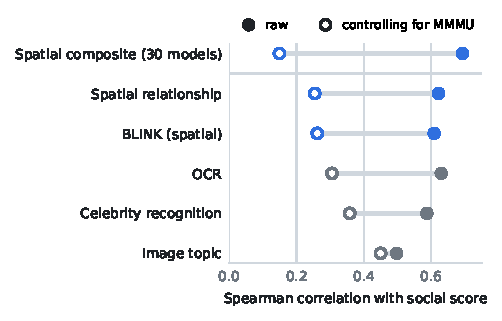
\includegraphics[width=\columnwidth]{lit_compact}
\caption{Correlation with social scores across published models, raw (filled) and controlling for MMMU (open). Top: spatial vs.\ social-reasoning composites (30 models). Below: MMBench Social Relation vs.\ spatial (blue) and non-spatial (grey) skills, 284 models, one evaluator. Spatial skills drop as much as unrelated ones.}
\label{fig:litscaling}
\end{figure}

\paragraph{Limitations.}
With $n{=}200$, effects below about 3 pp cannot be excluded. The probe labels come from the same extractors as the maps, and API results are single runs (GPT-5.6 agrees with itself on 83--90\% of items).

\subsection{Updated Research Idea}
\label{sec:idea5-updated}

\paragraph{What changes.}
Geometry is not the bottleneck: correct maps do no better than mismatched ones, and spatial training is neutral to harmful. The remaining errors concern people rather than space: most are perception failures about who is present, attending or approaching, and most condition effects are abstention. We therefore use body pose as a perception signal about people, integrated into the model rather than appended to its input.

\paragraph{Model.}
A human-centric pose encoder (e.g., Meta's Sapiens2) gives per-person keypoints, body orientation, gaze and an identity track over the five frames, projected to pose tokens $\mathbf p_k=W_p[\mathbf{kp}_k;\mathbf{orient}_k;\mathbf e_{\mathrm{id}(k)}]$ in Qwen3-VL-8B's width. Because extra sequence tokens distracted the models above, visual and language hidden states $\mathbf h$ read pose through gated cross-attention inserted every $n$ blocks,
\begin{equation}
\mathbf h\leftarrow\mathbf h+\tanh(\gamma)\,\mathrm{Attn}\big(W_q\mathbf h,\,W_kP,\,W_vP\big),\quad\gamma_0=0,
\end{equation}
so the base model is unchanged at initialisation and can ignore pose where it is uninformative. An InfoNCE alignment loss $\mathcal L_{\mathrm{align}}$ ties each $\mathbf p_k$ to the visual tokens inside person $k$'s mask, grounding pose in what the vision tower sees.

\paragraph{Training.}
We fine-tune on the norm objective $\mathcal L_{\mathrm{norm}}$ (cross-entropy on the gold action and justification) and add a counterfactual hinge that rewards using pose: with $s_\theta$ the log-probability of the gold answer and $\tilde P$ pose tokens from another clip, on items where facing or hand cues are informative,
\begin{equation}
\mathcal L_{\mathrm{cf}}=\textstyle\sum_{i\in S}\max\big(0,\,m-s_\theta(y_i\mid x_i,P_i)+s_\theta(y_i\mid x_i,\tilde P_i)\big).
\end{equation}
This turns our mismatched control into a training signal: a model that ignores pose cannot reduce it. A calibration term $\mathcal L_{\mathrm{abs}}$ penalises probability on ``None'' when a gold option exists. The objective is $\mathcal L_{\mathrm{norm}}+\lambda_1\mathcal L_{\mathrm{align}}+\lambda_2\mathcal L_{\mathrm{cf}}+\lambda_3\mathcal L_{\mathrm{abs}}$.

\paragraph{Evaluation.}
We keep the controls that made the current results interpretable: mismatched pose at test time, pose dropout (gates closed) and the same model trained on $\mathcal L_{\mathrm{norm}}$ alone, with at least two seeds, reporting high- vs.\ low-pose-need items, the ``None'' rate and forced-choice accuracy. The idea succeeds only if the pose model beats both the norm-only model and its own mismatched-pose arm; a gain that survives mismatched pose would again be a format or abstention effect.
